% Section content template for individual Educative lessons
% This file contains the actual content for a specific section
% Generated from Educative API section content

% Section: Getting Ready: An Online Stock Brokerage System
% Section ID: 5081333196128256
% Section Slug: getting-ready-an-online-stock-brokerage-system
% Generated: 2025-12-14T12:53:00.199171

\subsection{Problem definition}\label{8t8osGei0gD63dyNYRfeL-1}
\\
An \textbf{online stock brokerage} system acts as an intermediary between the buyer and seller during the trade of stocks. The system facilitates its users\textquotesingle{} buying and selling of stocks online. It enables users to monitor and carry out their transactions and displays performance graphs for the various stocks in their portfolios. It also protects client transactions and notifies them when stock changes reach certain levels.
\\
The online stock brokerage system streamlines traditional trading using digital infrastructure, offering faster transactions and reduced operational costs. It also offers users quicker access to stock information, market trends, and real-time prices. Additionally , the system supports deposits and withdrawals through checks, wire transfers, or electronic bank transfers, enhancing overall financial flexibility for users.

\begin{figure}[htbp]
 \centering
 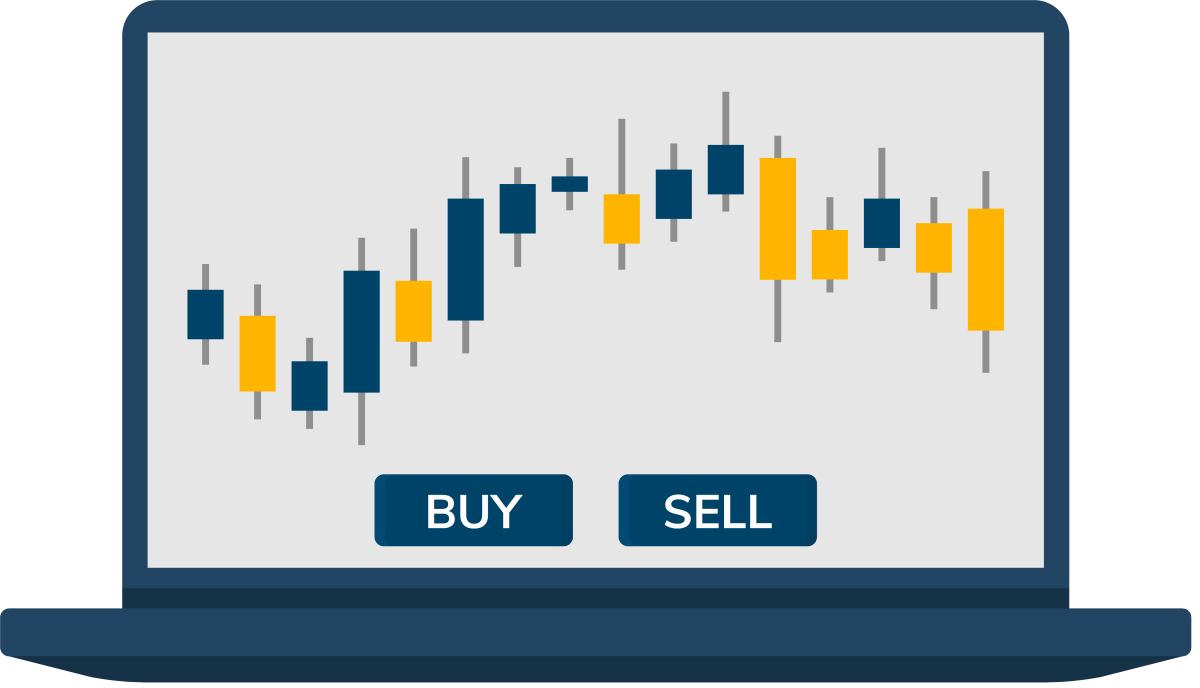
\includegraphics[width=0.15\textwidth]{Images/chapter_23/section_5081333196128256/4702351854403584.png}
 \caption{The online stock brokerage system}
\end{figure}

\subsection{Expectations from the interviewee}\label{8t8osGei0gD63dyNYRfeL-2}
\\
An online stock brokerage system consists of multiple components. Each component has its own functionality and constraints. The following section provides an overview of some of the main expectations the interviewer will want to hear you discuss in more detail during the interview.

\subsubsection{Discoverability}\label{iLkfZzbpdr5NER2btESOI}
\\
For an online stock brokerage system, discoverability is one of the key features. You can ask the following questions to know more about the system:

\begin{itemize}
\item
\protect\phantomsection\label{8U3-KUlQSLnj94TEBU0vp}
How do the members search the stock inventory?
\item
\protect\phantomsection\label{LE82gxTZt4_7y_4Ou4gVh}
How will the search surface result?
\end{itemize}

\subsubsection{Visibility}\label{h0yykrFO5tS6Tl0PtLlY3}
\\
To get a better understanding of how the data is visible to the different users, you may ask the following questions:

\begin{itemize}
\item
\protect\phantomsection\label{VXqSXjI2reO6aR8EEP783}
Can every member see the current levels of stock positions at any time?
\end{itemize}

\subsubsection{Order type}\label{NV9FEg5EzfR6z5DY0IKgt}
\\
You may ask the interviewer about the types of orders the system should be able to handle by simply asking the question listed below:

\begin{itemize}
\item
\protect\phantomsection\label{g8EQ18cIzNXkbbdcNt9FL}
How many types of stock trade orders can the users place, for example, a market order, loss order, etc?
\end{itemize}

\subsubsection{Multiplicity}\label{mtTy2Q_Wy__Jr1NHohniL}
\\
You may ask the interviewer questions related to the multiplicity of the system. These questions are listed below:

\begin{itemize}
\item
\protect\phantomsection\label{NSbYz7wsqa-iA6GOteE2h}
Can the members have multiple watchlists containing multiple stock quotes?
\item
\protect\phantomsection\label{QeHuLTgHQTcOcnvsbzIcM}
Can a member buy multiple lots of the same stock at different times?
\end{itemize}

\subsection{Design approach}\label{AvFkqX_uBnryIUoPxD7XV}
\\
We'll design this online stock brokerage system using the bottom-up design approach. For this purpose, we will follow the steps below:

\begin{itemize}
\item
Identify and design simple components, like stock and stock position, first.
\item
Use these small components to design bigger components, such as the order and stock inventory, which can be composed of multiple stock items.
\item
Repeat the steps above until we design the whole stock brokerage system.
\end{itemize}

\subsection{Design pattern~}\label{I9TiD23Ux3o1GCM4ZFKky}
\\
During an interview, discussing the design patterns that an online stock brokerage system falls under is always a good practice. Stating the design patterns gives the interviewer a positive impression and shows that the interviewee is well-versed in the advanced concepts of object-oriented design.
\\
Try to answer the following question. If you are not familiar with design patterns, don't worry! You can learn about them by asking ``Define design patterns.''

\textbf{Question:}

Which design pattern(s) should be used to design an online stock brokerage system? Please elaborate on your choice(s).

Let's explore the requirements of the online stock brokerage system in the next lesson.

% End of section content